%!TEX root = ../thesis.tex

\section{Introduction}

%Hung-yi Lee: I think maybe we need a basic frame image. I happen to have an image that can be used here.
\begin{figure}
    \centering
    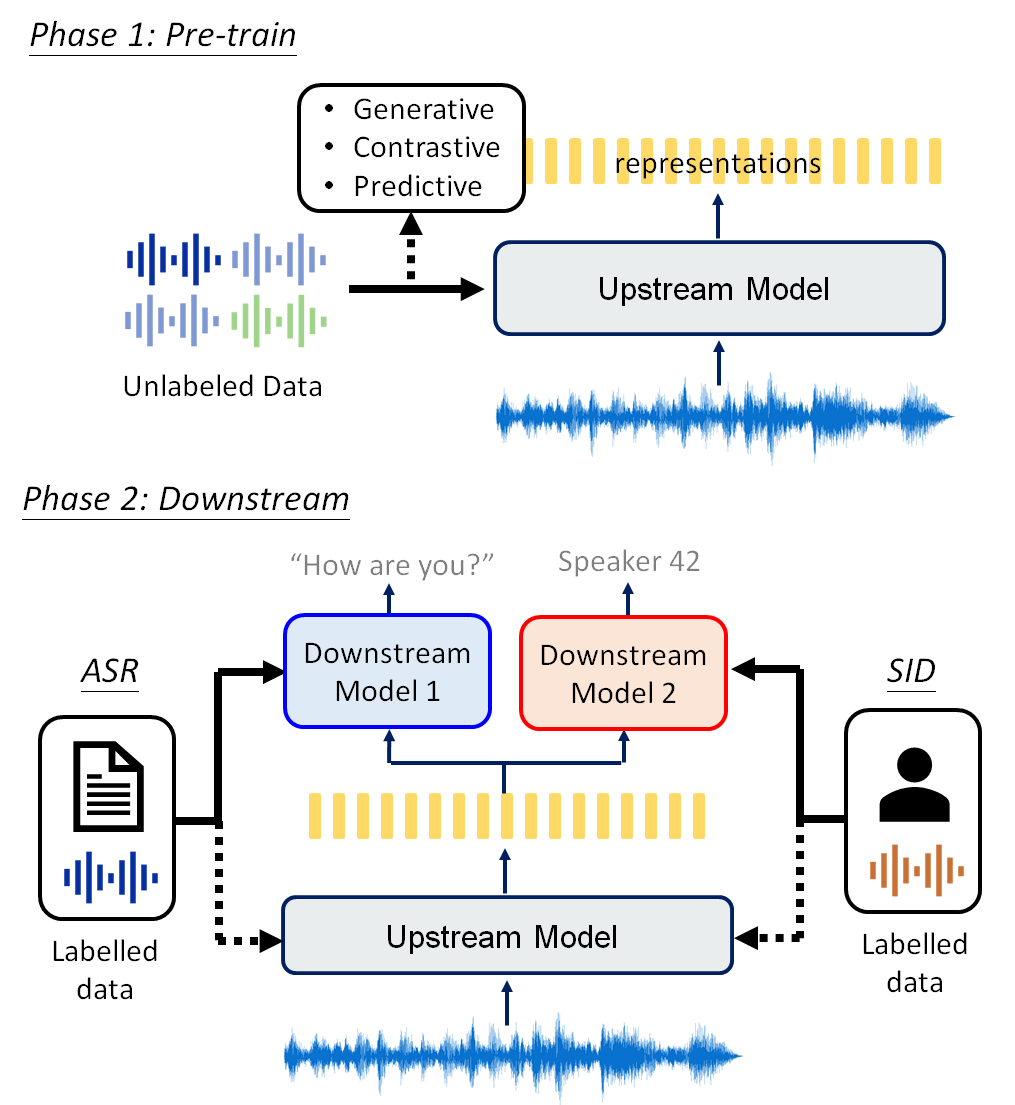
\includegraphics[width=0.80\textwidth]{paper_review/SSL_framework.png}
	 \caption{Framework for using self-supervised representation learning in
	 downstream applications}
    \label{fig:SSL_framework}
\end{figure}

% {\color{blue} Reviewer: Daniel, KL, SW}\\
% {\color{blue} Abdo -- this section is a work-in-progress}\\

% {\color{red} Hung-yi: Last time we have decided to use "pre-train" (with "-")} -- Done\\

% {\color{red} Hung-yi: Fine-tune? or finetune?} --Fine-tune Done\\

% {\color{red} Hung-yi: Fig. 1 or Figure 1} -- Fig. 1  Done\\

% \abdo{comment from Shinji: bring references to intro.}

% \kl{Comments from Nov. 10 meeting: 
% \begin{itemize}
%     \item \abdo{added.} would be good to define representation learning a bit more thoroughly in the intro, and mention that we are considering both discrete and continuous representations.
%     \item \abdo{added.} it would also be good to mention and broadly define "self-supervised" in the intro (as of now it's first mentioned in Section~\ref{sec:thirdwave}), and mention that the term is now used (and we use it) for some techniques that in the past would have just been called "unsupervised".
% \end{itemize}}

% \kl{New comments: 
% \begin{itemize}
%     \item It would be good to include somewhere in the paper a summary of tasks for which SSL pre-trained models have the SOTA performance.  Maybe it is in the paper already but I don't see it.
% \end{itemize}}

Over the past decade, deep learning approaches have revolutionized speech processing
through a giant leap in performance, enabling various real-world applications.
Supervised learning of deep neural networks has been the cornerstone of this
transformation, offering impressive gains for scenarios rich in labeled
data~\cite{lecun2015deep, hinton2012deep, bourlard2012connectionist}. 
Paradoxically, this heavy reliance on supervised learning has restricted progress in
languages and domains that do not attract the same level of labeling
investment. 
%Paradoxically, the heavy reliance on supervised learning bottlenecked the development of novel industrial speech applications and restricted progress in languages and domains that do not entertain the same level of labeling investment. 

To overcome the need for labeled data, researchers have explored approaches that use
unpaired audio-only data to open up new industrial speech use-cases and
low-resource languages~\cite{Kemp1999, csl01_limsi, ma_bbn_06}. Inspired by how
children learn their first language through listening and interacting with
family and surroundings, scientists seek to use raw waveforms and
spectral signals to learn speech representations that capture low-level
acoustic events, lexical knowledge, all the way to syntactic and semantic
information. These learned representations are then used for target downstream
applications requiring a minimal number of labeled data~\cite{Hinton_2007,
LeCun06atutorial, bengio_representation_2013}. 
Formally, representation learning refers to algorithms for extracting latent
features that capture the underlying explanatory factors for the observed
input~\cite{bengio_representation_2013}. 
% Previous research efforts explored latent representations that are binary \cite{}, discrete \cite{} and continuous \cite{}. 
% These latent representations are generally used as inputs to a supervised predictor or a generation module. The whole network generating these representations is frequently used to initialize a supervised classifier~\cite{hinton_2006}. 

%Learning representations approaches generally fall within \textit{unsupervised learning}, which refers to the family of machine learning methods that discover naturally occurring patterns in the training samples without any pre-assigned labels or scores associated with these samples~\cite{jordan_2015}. 
Representation learning approaches are generally considered examples of \textit{unsupervised
learning}, which refers to the family of machine learning methods that discover
naturally occurring patterns in training samples for which there are no pre-assigned
labels or scores~\cite{jordan_2015}. 
The term ``unsupervised'' is used to distinguish this family of methods from
``supervised'' approaches, which assign a label to each training sample, and
``semi-supervised'' approaches, which utilize a small number of training samples
with labels to guide learning using a larger volume of unlabeled samples.
Examples of unsupervised learning techniques include k-means clustering~\cite{vq}, mixture models~\cite{MoE}, autoencoders~\cite{hinton_94},
and non-negative matrix factorization~\cite{nmf}. 
\textit{Self-supervised learning} (SSL) is a fast-growing subcategory of
unsupervised learning approaches, which are techniques that utilize
information extracted from the input data itself as the label to learn
representations useful for 
% one or many 
downstream tasks. {\color{black} For example, unsupervised k-means clustering doesn't adhere to this definition of self-supervision since it iteratively minimizes the within-cluster variance during learning.}
In this review, we
focus on self-supervised learning approaches.

\Cref{fig:SSL_framework} outlines self-supervised representation learning in
relation to downstream applications. 
There are two stages in this framework.
In the first stage, we use SSL to pre-train a \textit{representation model},
also called an \textit{upstream model} or a \textit{foundation model}.
In the second stage, downstream tasks use either the learned
representation from the frozen model, or fine-tune the entire pre-trained model
in a supervised phase~\cite{hinton_2006}. 
%e.g., Automatic Speech Recognition (ASR) and Speaker Identification (SID) are two example downstream applications in \cref{fig:SSL_framework}. 
Automatic speech recognition (ASR) and speaker identification (SID) are 
examples of downstream applications in \cref{fig:SSL_framework}.
% There are some task-specific labeled data for each downstream task, and there is a downstream model on top of the upstream model. The labeled data is used to train the corresponding downstream models and optionally fine-tune upstream models.
% If the pre-training stage only leverages unlabeled data, the framework in \cref{fig:SSL_framework} is named self-supervised learning (SSL), which is the focus of this review paper.
% Pre-training with labeled data is out of the scope. Before the term self-supervised learning was widely used, pre-training without any labeled data was usually known as an \texit{unsupervised learning} approach. 




%Lee: in the introduction, we may need a specific example. Below is just an example.
%With unsupervised ASR, imagine that in the future, when an indigenous language family buys an intelligent assistant, even if the assistant does not support the language at the beginning, it would automatically learn to transcribe the new language after learning.



% The speech representation learning approaches evolved over the past few decades through at least three major stages, as discussed in \cref{sec:thirdwave}; static and temporal clustering algorithms \cite{}, energy-based neural models \cite{}, and more recently, self-supervised learning techniques \cite{}. 
% Across all these three waves of representation learning, three main desirable characteristics emerged; features need to be disentangled, invariant, and hierarchical. 
It is considered desirable for learned speech representations to be
disentangled, invariant, and hierarchical.
Since spoken utterances contain much richer information than the corresponding text
transcriptions---e.g., speaker identity, style, emotion, surrounding noise, and
communication channel noise---it is important to learn representations that
disentangle these factors of variation. Furthermore, invariance of the learned
features to changes in background noise and in the communication channel ensures
stability with respect to downstream application scenarios. Learning feature
hierarchies at the acoustic, lexical, and semantic levels supports applications
with different requirements. For instance, whereas a speaker identification task
benefits from a low-level acoustic representation, a speech
translation task requires a more semantic representation of the input
utterance. 

Due to the popularity of SSL, reviews have been published about the
technology in general~\cite{bommasani2021opportunities,ericsson2021selfsupervised,LiuSSLsurvey} as well as its application to natural language processing (NLP)~\cite{rogers-etal-2020-primer,liu2021pretrain,xia-etal-2020-bert,QiuSSLNLPsurvey} and computer vision (CV)~\cite{JingSSLCVsurvey}. Recently, a brief overview with a general focus on speech representation learning was published \cite{borgholt_22}. However, none of these overviews focus exclusively on SSL for speech processing. Since the speech signal differs greatly from image and text inputs, many  theories  and technologies have been developed to address the unique challenges of speech. One review addresses speech representation learning based on deep learning models~\cite{latif2021deep}, but does not address recent developments in self-supervised learning. This motivates this overview of speech SSL.


%For survey papers on TL to speech processing, please check the reference~\cite{survey_speech_TL}.
%The representation learning methods covered in this review are primarily task-agnostic methods that only benefit from supervised data at the fine-tuning stage, as shown in \cref{}. %Lee: Similar sentence may have been mentioned in the paragraph describing the figure.

The structure of this paper is arranged as follows. \Cref{sec:thirdwave}
briefly reviews the history of speech representation learning, and
\cref{sec:approach} reviews current speech SSL models.
\Cref{section:benchmark} surveys SSL datasets and benchmarks, 
and discusses and compares results from different works. \Cref{analysis}
analyzes successful SSL approaches and offers insights into the
importance of technological innovations. \Cref{sec:zero} reviews 
zero-resource downstream tasks that utilize SSL. 
Finally, \cref{sec:conclusion} summarizes the paper and suggests 
future research directions.


